    \subsection*{Initializing the $k$-means algorithm}
    
        Now that we have our \textbf{clusters}, \textbf{means}, and a \textbf{loss} function for evaluating them, we can begin looking for a better \textbf{clustering}.
        
        We'll start out with a \textbf{dataset} we want to cluster: we'll use the one from the \textbf{beginning} of the chapter:
        
        \begin{figure}[H]
            \centering
            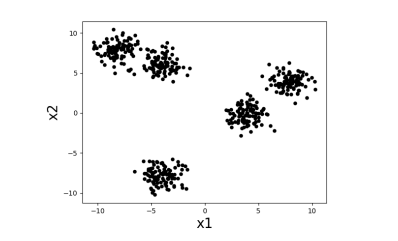
\includegraphics[width=70mm,scale=0.4]{images/clustering_images/clustering_example.png}
            \caption*{We could cluster this visually, but we want our machine to be able to do it for us.}
        \end{figure}
        
        First, we need to decide on our \textbf{number} of clusters. When you can't \textbf{visualize} it, this can be \textbf{difficult} - how many is too many or too few? 
        
        But, for now, we'll \textbf{ignore} that problem, and say $k=5$. 
        
        Let's \textbf{randomly} assign our initial cluster means, and assign each point to the \textbf{closest} cluster:
        
        \begin{figure}[H]
            \centering
            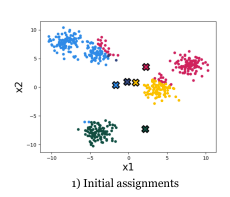
\includegraphics[width=70mm,scale=0.4]{images/clustering_images/initialization_cluster.png}
            \caption*{This is our starting point for the algorithm.}
        \end{figure}
    
    \subsection*{First step: moving our cluster means}
    
        As we mentioned before, these points aren't \textbf{actually} the average of their cluster: you can tell that by looking at it.
        
        We want to \textbf{minimize} the variation in our cluster: that's why we're using the mean.
        
        So, let's fix this: we'll take the \textbf{average} of all the points in each \textbf{cluster}, and \textbf{move} the cluster mean to that position.
        
        \begin{figure}[H]
            \centering
            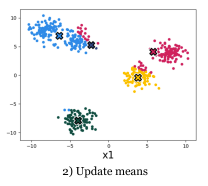
\includegraphics[width=70mm,scale=0.4]{images/clustering_images/update_means_clustering.png}
        \end{figure}
        
        And now, our cluster means are closer to all our data points!\\
        
        \begin{concept}
            One way \vocab{minimize} the \vocab{distance} between the \purp{cluster mean} and its \gren{data points} is:
            
            \begin{itemize}
                \item Take the \gren{average} of all the points in the cluster, and \purp{reassign} the cluster mean to that average.
            \end{itemize} 
        \end{concept}
        
    \subsection*{Second step: Reassign data points}
    
        We've \textbf{improved} our model by moving the cluster mean.
        
        The problem is, we originally \textbf{assigned} every point to the \textbf{closest} cluster mean. 
        
        If the cluster means \textbf{move}, then some points might be closer to a \textbf{different} cluster now!
        
        If so, we can \textbf{improve} our clustering further by reassigning points to the cluster they're \textbf{closest} to!
        
        \begin{figure}[H]
            \centering
            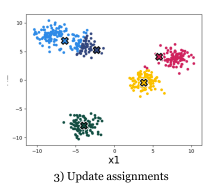
\includegraphics[width=70mm,scale=0.4]{images/clustering_images/update_assignments_clustering.png}
        \end{figure}\\
        
        \begin{concept}
            Another way \vocab{minimize} the \vocab{distance} between the \purp{cluster mean} and its \gren{data points} is:
            
            \begin{itemize}
                \item After the \purp{means} have been \gren{moved}, \vocab{reassign} the \vocab{data points} to whichever mean is \purp{closest}.
            \end{itemize} 
        \end{concept}
        
    \subsection*{The cycle continues}
    
        But wait - now that we've changed the points in each cluster, our cluster mean might not be the \textbf{true} average!
        
        So, we can, again, improve our loss by taking the average of each cluster, and moving the cluster mean.
        
        This creates a cycle that continues until we \textbf{converge} on our final answer.\\
        
        \begin{concept}
            Together, of our steps for \gren{improving} our clusters create a \vocab{cycle} of \purp{optimization}:
            
            \begin{itemize}
                \item \purp{Moving} our cluster mean \gren{changes} which point should go in each cluster.
                
                \item \purp{Reassigning} points to different clusters \gren{changes} our cluster mean.
            \end{itemize}
        \end{concept}
        
    \subsection*{The $k$-means algorithm}
    
        These two steps make up the \textbf{bulk} of our algorithm:\\
        
        \begin{definition}
            The \vocab{$k$-means algorithm} uses the following steps:
            
            \begin{itemize}
                \item First, we \purp{randomly} choose our \gren{initial} cluster means.
            \end{itemize} 
            
            Then, we \purp{cycle} through the following two steps:
            
            \begin{itemize}
                \item \purp{Reassign} \gren{points} to the cluster mean they're closest to.
                
                \item \purp{Move} each \gren{cluster mean} to the average of all the points in that cluster.
            \end{itemize}
            
            Until our clusters means \purp{stop} changing.
        \end{definition}
        
        When we run our algorithm on the above dataset, we get:
        
        \begin{figure}[H]
            \centering
            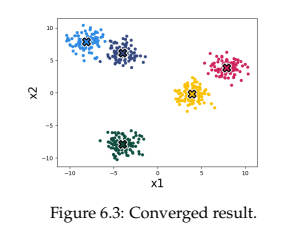
\includegraphics[width=70mm,scale=0.4]{images/clustering_images/converged_result_clustering.png}
        \end{figure}
        
        Note that, our cycle \textbf{works} because changing \textbf{either} cluster mean or point assignments allows you to further \textbf{improve} the \textbf{other} step.
        
        So, if we're \textbf{not} changing one of them, the other one won't \textbf{change} either: the cycle is \textbf{broken}, and we can \textbf{stop}. 
            \note{This is our termination condition!}
        
        Another nice fact: it can be shown that this algorithm does \textbf{converge} to a local minimum!\\
        
        \begin{concept}
            The \vocab{$k$-means algorithm} is guaranteed to \purp{converge} to a \gren{local minimum}.
        \end{concept}
        
    \subsection*{Pseudocode}
    
        \begin{codebox}
          \Procname{$\proc{k-means}(k, \tau, \{x^{(i)}\}_{i=1}^n)$}
          \li $\mu, y \gets $ randinit  \qquad\#Random initialization
          \li \For $t \gets 1$ \To $\tau$   \qquad\#Begin cycling
          \li
          \li   \Do
                 $y_{\texttt{old}} = y$ \qquad\#Keep track of last step
                 
          \li
          \li        \For $i \gets 1$ \To $n$
          \li       \Do
                     $y^{(i)} = \arg\min_j \left\Vert x^{(i)} - \mu^{(j)} \right\Vert_2^2$
                     \qquad\#Reassign data point to closest mean
                    \End
                    
          \li
          \li    \For $j \gets 1$ \To $k$
          \li       \Do 
                     $\mu^{(j)} = \frac{1}{N_j} \sum_{i=1}^n \mathbb{1}(y^{(i)} = j) x^{(i)}$
                     \qquad\#Move cluster mean to average of cluster
                    \End
                    
        \li
          \li      \If $\mathbb{1}(y = y_{\texttt{old}})$
          \li          \Then
        		  break \qquad\#If nothing has changed, then the cycle is done. Terminate
              \End
              \End
          \li
          \li \Return $\mu, y$
        \end{codebox}